\documentclass{beamer}
\usepackage[utf8]{inputenc}
\usepackage{graphicx}
\usepackage[export]{adjustbox}

\title{\textbf{ECSE-487 \\ Digital Storage Oscilloscope \\ Mid-term presentation}}
\author{Andrei Purcarus \and Ze Yu Yang}
\date{March 13, 2017}

\begin{document}

\maketitle

\begin{frame}
\frametitle{Digital Storage Oscilloscope - Overview}

\begin{figure}[!htb]
  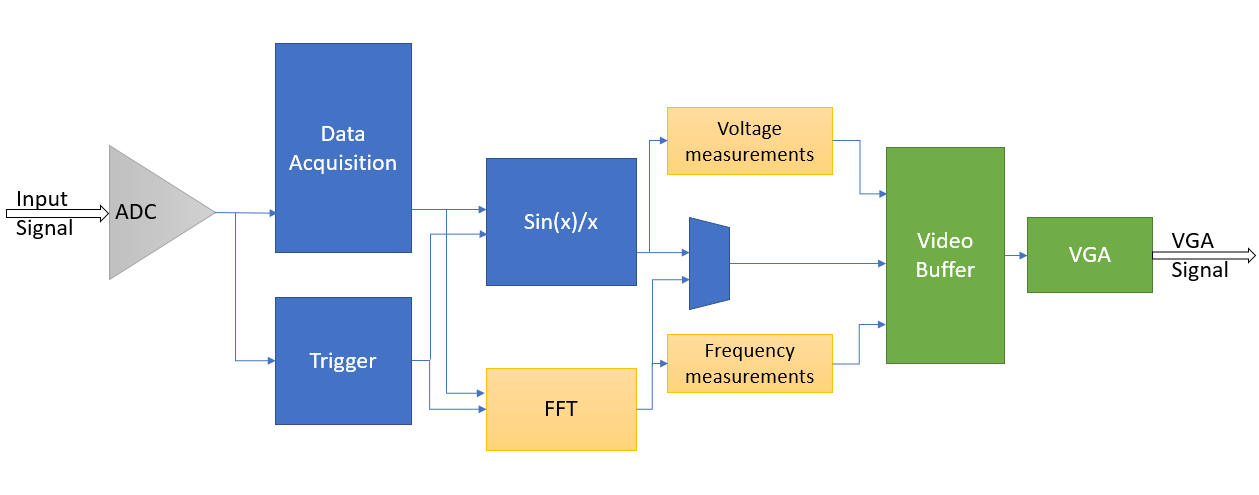
\includegraphics[width=\linewidth]{system_diagram.png}
\end{figure}

\end{frame}

\begin{frame}
\frametitle{VGA Module - Overview}

\begin{figure}[!htb]
  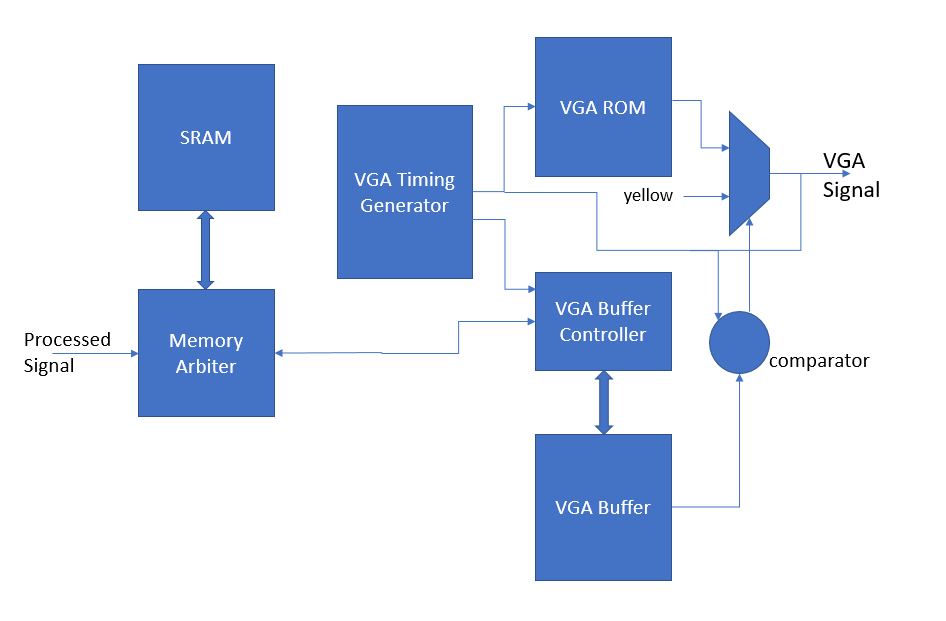
\includegraphics[width=\linewidth]{VGA_diagram.png}
\end{figure}

\end{frame}

\begin{frame}
\frametitle{VGA Timing Test Results}

\begin{columns}[onlytextwidth]
  \begin{column}{0.5\linewidth}
  
  	\begin{figure}[!htb]
      
\includegraphics[width=\linewidth]{vga_timing_test_result.png}
	\end{figure}
    
  \end{column}
  \begin{column}{0.45\linewidth}
  
  	\begin{itemize}
      \item A testbench was used to generate color bars based on ROW and COLUMN.
      \item The VGA output was displayed using a simulator.
	\end{itemize}
    
  \end{column}
\end{columns}

\end{frame}

\begin{frame}
\frametitle{VGA Background Image Test Results}

\begin{columns}[onlytextwidth]
  \begin{column}{0.5\linewidth}
  
  	\begin{figure}[!htb]
      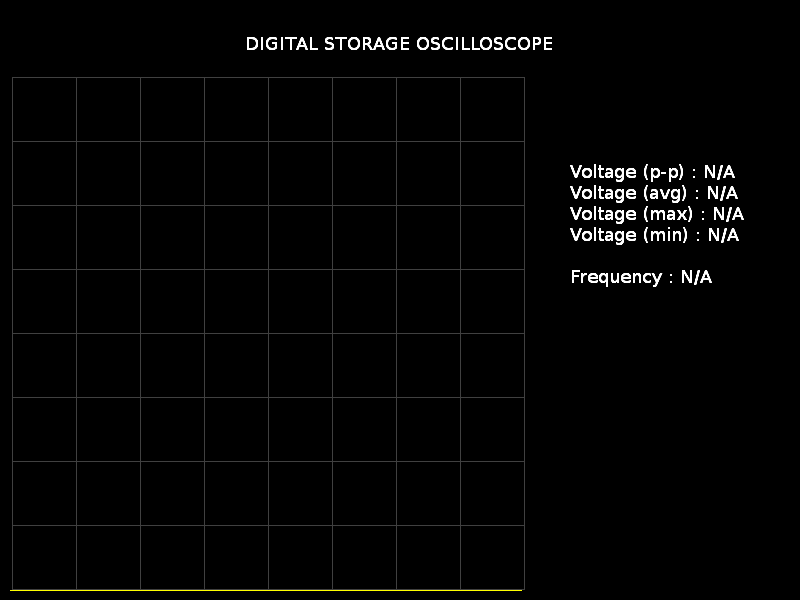
\includegraphics[width=\linewidth]{vga_background_test_result.png}
	\end{figure}
    
  \end{column}
  \begin{column}{0.45\linewidth}
  
  	\begin{itemize}
      \item The background image file was loaded into the ROM.
      \item The VGA output was displayed using a simulator.
	\end{itemize}
    
  \end{column}
\end{columns}

\end{frame}

\begin{frame}
\frametitle{VGA Test Signal Results}

\begin{columns}[onlytextwidth]
  \begin{column}{0.5\linewidth}
  
  	\begin{figure}[!htb]
      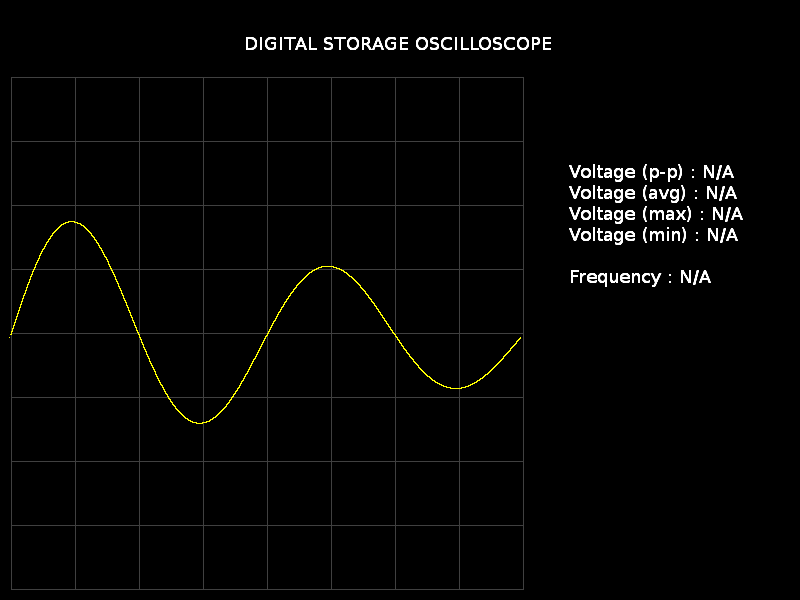
\includegraphics[width=\linewidth]{vga_test_signal1_results.png}
	\end{figure}
    
  \end{column}
  \begin{column}{0.45\linewidth}
  
  	\begin{itemize}
      \item The test signal was loaded into the SRAM.
      \item The VGA output was displayed using a simulator.
	\end{itemize}
    
  	\[ f(t) = sin( {2 \pi t}/{T} ) e^{{-t}/{2 T}} \]
    
  \end{column}
\end{columns}

\end{frame}

\begin{frame}
\frametitle{VGA Test Signal Results}

\begin{columns}[onlytextwidth]
  \begin{column}{0.5\linewidth}
  
  	\begin{figure}[!htb]
      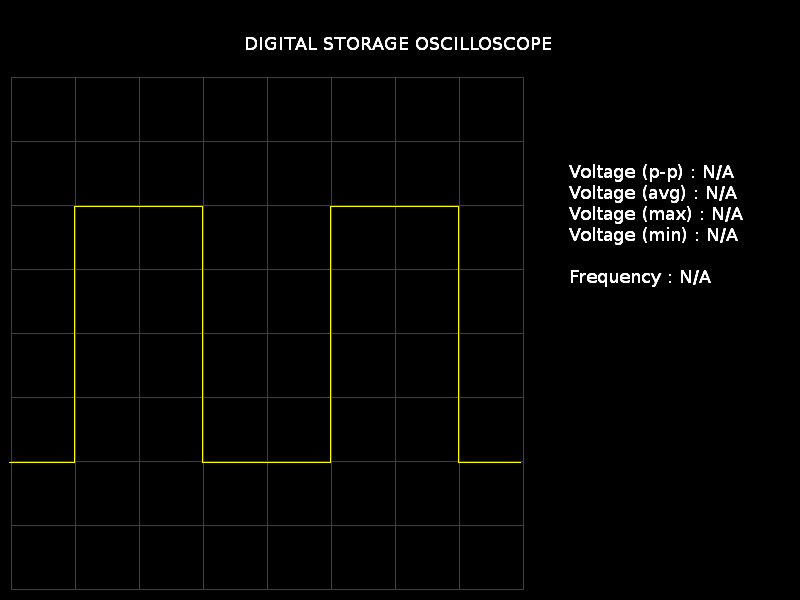
\includegraphics[width=\linewidth]{vga_test_signal2_results.png}
	\end{figure}
    
  \end{column}
  \begin{column}{0.45\linewidth}
  
  	\begin{itemize}
      \item The test signal was loaded into the SRAM.
      \item The VGA output was displayed using a simulator.
	\end{itemize}
    
  	\[ f(t) = square(2 \pi t / T) \]
    
  \end{column}
\end{columns}

\end{frame}

\end{document}
